\documentclass[11pt,a4paper]{article}
\usepackage[latin1]{inputenc}
\usepackage[spanish,activecute]{babel}
\usepackage{amsmath}
\usepackage{amsfonts}
\usepackage{amssymb}
\usepackage{graphicx}
\usepackage[left=2cm,right=2cm,top=2cm,bottom=2cm]{geometry}
\title{LINEA DE PRODUCCION}
\author{MEJORADA LOPEZ IVAN\\TORRES PINTO LUIS ANGEL\\ALVAREZ SOTELO GABREIL\\VARGAS DIAZ MARCO ANTONIO}
\\
\begin{document}
\maketitle


\includegraphics[width=\textwidth]{UPZMG_Prueba_1b.png} 
\newpage
\section{Introduccion}
Los alumnos de 4B de la carrera ingenieria en mecatronica decidimos hacer este proyecto ya que nos podria servir en un futuro para saber como operar y usasr una linea de produccion, en este proyecto pondremos todas nuestas capacidades y todo nuestro conocimiento, es un proyecto a largo plazo el plazo para lograrlo es de un a\~no, en este a\~no dise\~naremos el proyecto y perfeccionaremos cada punto que se nos comente por las diferentes asignaturas involucradas con el proyecto.\\En este proyecto mostraremos sobre el avance de nuestra linea de prodducion el cual tendra involucradas varias materias, sera automatizado sobre una banda,y carios motores para ello neceistermos los diguientes materiales que se mencionanan en seguida 
\\
\\
\section{MATERIALES}
electrovalvula\\motor de dos sensores de precencia\\plc\\banda\\tabla\\botones\\leds\\visagras\\soportes\\caja de acrilico\\cervomotores\\material que se necesita para dispersar(arroz)
\\
\section{OBJETIVO GENERAL, A DONDE QUEREMOS IR}
El objetivo general del proyecto es dise\~nar y elaborar una linea de produccion que sea mas eficaz
al momento de producir y verificar que la linea tenga mejor desempe\~no en cuanto productividad,
asi como verificar su dise\~no y rendimiento para que sean mejores, por ello necesitaremos
corroborar que nuestra linea de produccion propone algo mejor en la produccion. Teniendo esto
en nuestra nuestro proyecto estara terminado.
\subsection{OBJETIVOS DEL PROYECTO}
1.DISE\~NAR NUESTRA LINEA DE PRODUCCION\\2.CORRER LA LINEA DE PRODUCCION\\3.SOLUCIONAR PROBLEMAS ADICIONALES QUE TENGA NUESTRA LINEA DE PRODUCCION\\4.EVALUAR LA FACTIBILIDAD Y EFICIENCIA QUE TENGA NUESTRO PROYECTO\\5.VERIFICAR QUE EL DESEMPE\~NO SEA ADECUADO\\6.PROPONER MEJORADA PARA LA LINEA DE PRODUCCION TENGA MEJORES QUE LAS DE PROCESO 
\newpage
\section{PLANTEAMIENTO DEL PROBLEMA}
El gran incremento en produccion, ha producido un problema en el resultado y desempe\~no del
proceso de fabricacion de un producto, asi mismo los costos de mantenimiento los cuales son muy
elevados. A la hora de hablar de la eficiencia y productividad del proceso de una industria esta se
queda muy corta, ya que el desempe\~no en sus lineas de produccion no es el correcto o las
operaciones del proceso no son del todo adecuadas.\\Por ello nosotros queremos solucionar el problema creando una linea de produccion
automatizada, con el fin de tener un buen resultado con el producto final y que sea mas rapido
que una linea de produccion normal, y que asi mismo el mantenimiento del proceso no sea tan
elevado.
\\
\section{MATERIAS INVOLUCRADAS EN EL PROYECTO }
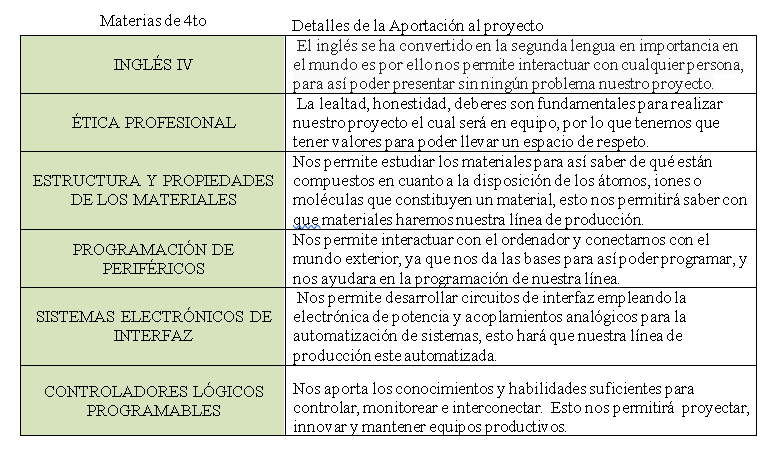
\includegraphics[scale=0.5]{71145735_653968975091118_3870654209674182656_n.png} \\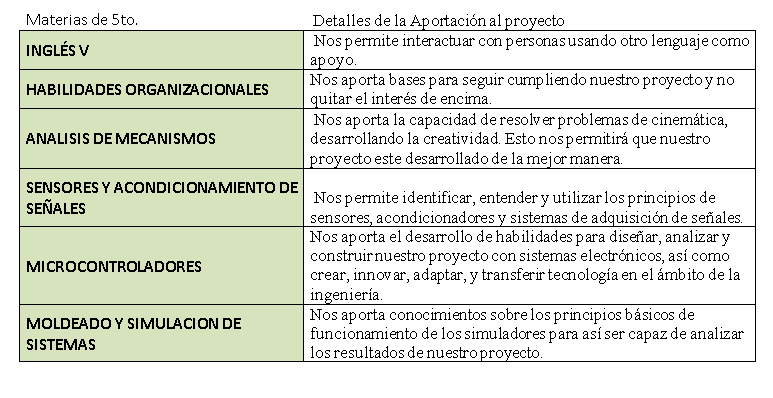
\includegraphics[scale=0.5]{71089516_2412079752447274_7094167623637663744_n.png} 
\newpage

\\
\\



\section{JUSTIFICACI\'ON}
Este proyecto lo llevamos acabo por el echo de demostrar una peque\~na parte de un proceso de industria en este demostraremos como se basan las empaquetadoras de arroz, las empresas mas grandes tienen maquinas como la de este proyecto mucho mas grandes, podemos ver en la imagen [1] como son las empresas de arroz.\\En la imagen[2] podremos observar un voceto en el cual nosotros nos basaremos para terminar nuestro proyecto.\\Tambien podremos ver los procesos que lleva el proyecto desde el armado hasta quedar terminado. 
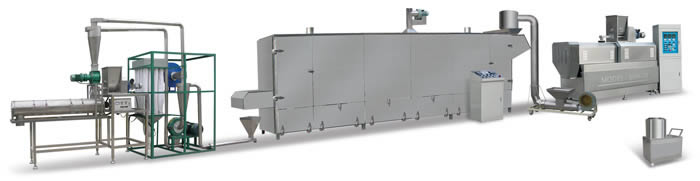
\includegraphics[width=\textwidth]{12-1-1b.jpg}
\\
\\ 
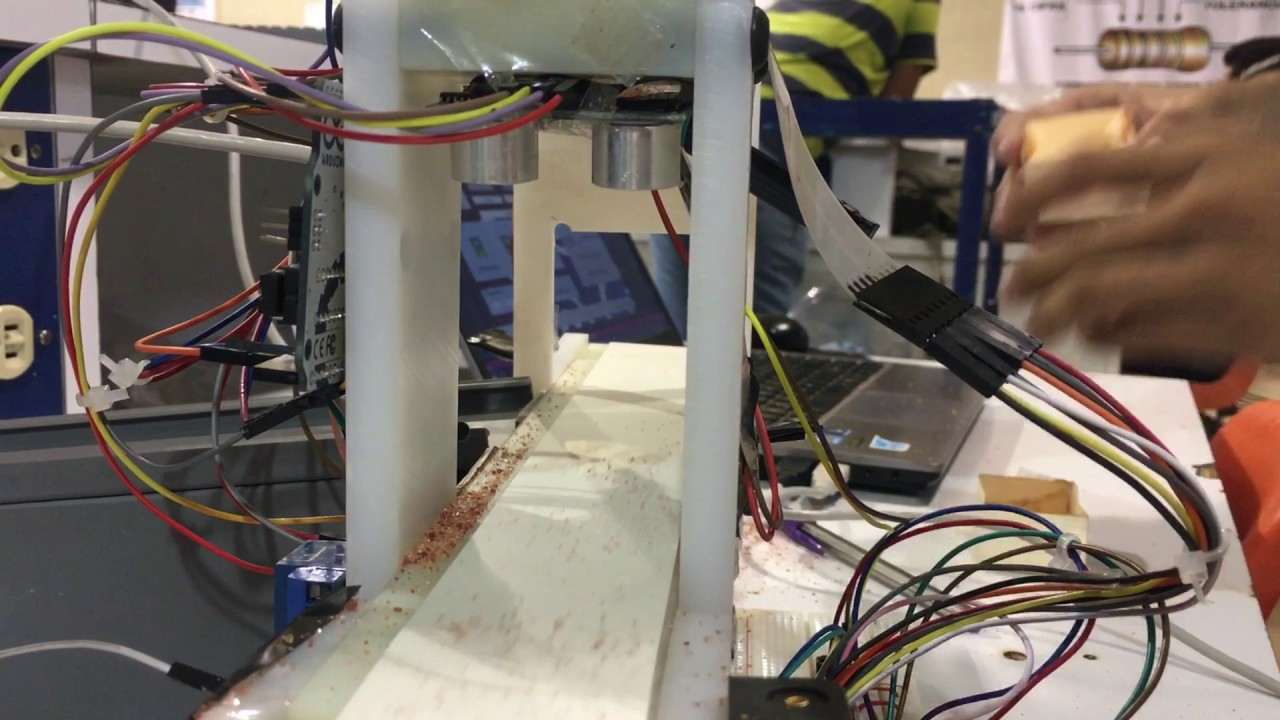
\includegraphics[width=\textwidth]{imagen2.jpg} 
\newpage
\section{DIAGRAMA DE GANTT}
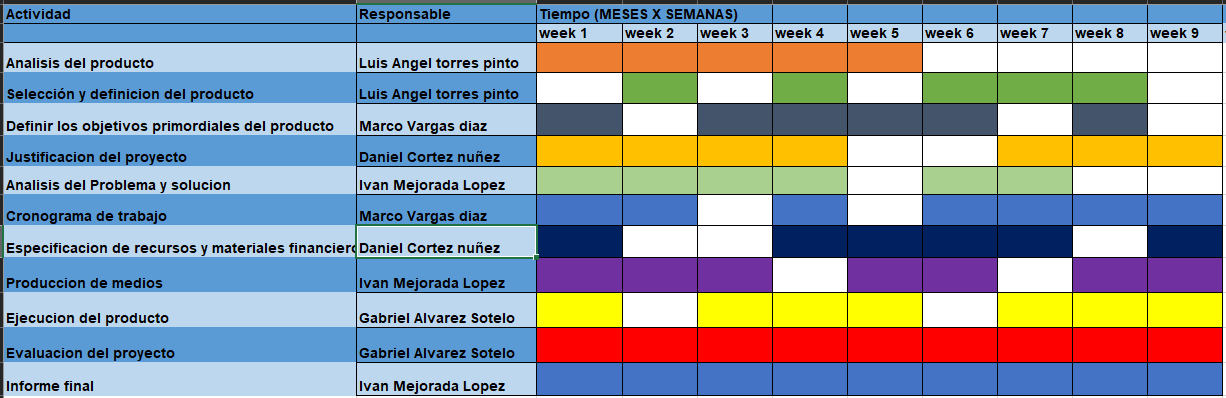
\includegraphics[width=\textwidth]{diagrama de gant.png} 








\end{document}